\section{Analytical Hidden Input Observability}

We consider the mapping $L^2([0,T])^{\otimes m}\to L^2([0,T])^{\otimes p}$ defined by 
\begin{equation}
y(t) := C \int\limits_0^t \e^{A(t-\tau)} D w(\tau) \, \td \tau \label{eq:y}
\end{equation}
where $w:[0,T]\to \mathbb{R}^m$, $y:[0,T]\to \mathbb{R}^p$, $A\in\mathbb{R}^{n\times n}$, 
$D\in\mathbb{R}^{n\times m}$ and $C\in\mathbb{R}^{p\times n}$. \\

We assume that in biological systems the functions $w$ and $y$ are defined on 
a natural interval of time that covers $[0,T]$. This means, that for a small $\epsilon$ the 
model could be extended to an interval $(0-\epsilon , T+\epsilon)$ and thus differentiation 
of $w$ and $y$ at $t=0$ and $t=T$ makes sense. To denote this idea without 
introducing $\epsilon$ we use the notation $[0^-,T^+]$.
\\

For any function $f(t,\tau)$ it is easy to see that
\begin{equation}
	\frac{\td}{\td t} \int\limits_0^t f(t,\tau) \, \td\tau = \int\limits_0^t
	\frac{\partial f}{\partial t}(t,\tau)\,\td\tau + f(t,t) \quad . 
\end{equation}
Using the latter equation we get the derivatives of $y$ as
\begin{equation}
	y^{(q+1)}(t) = CA^{q+1} \int\limits_0^t \e^{A(t-\tau)} D w(\tau) \, \td \tau + 
	\sum\limits_{l=0}^q  CA^lD w^{(q-l)}(t) \label{eq:y_derivatives}
\end{equation}
where $y^{(q+1)}$ denotes the $q+1$-st derivative and analogous for $w$.

\begin{definition}{}{}
	We write
	\begin{enumerate}
	\item $M_q := \left[ (CA) \,(CAD) \, \ldots \, (CA^qD) \right]$ and 
	$V_q :=\kernel{M_q}$. 
	\item $P:\mathbb{R}^{(q+1)m}\to \mathbb{R}^{qm}$ is the "projection" operator that 
	cuts away the first $m$ components of a vector. 
	\item $\mathfrak{O}_{l,d} := \bigcap\limits_{q=0}^l P^q V_{d+q}$ 
	and $\mathfrak{O}_d:= \lim\limits_{l\to \infty} \mathfrak{O}_{l,d}$.
%	\item $\mathfrak{D}_q:= \bigcap\limits_{l=0}^q P^{-l}V_{q-l}$ and 
%	$\mathfrak{D}:=\lim\limits_{q\to\infty} \mathfrak{D}_q$
	\item $W^{(q,r)}(t):=\left[ w^{(q)}(t) ,w^{(q-1)}(t),\ldots ,w^{(r)}(t)
	 \right]^\text{T}$ as a column vector. 
	 \item $W^{(q)}:=W^{(q,0)}$.
	\end{enumerate}
\end{definition}

\begin{remark}{}{}
	\begin{itemize}
	\item $M_q$ is understood as a concatenation of $p\times m$ matrices. Therefore it is 
	a $p\times (q+1)m$ matrix.	
	\item	
	Also note that $V_{r}\subseteq\mathbb{R}^{(r+1)m}$ and therefore also 
	$\mathfrak{O}_{q,r} \in \mathbb{R}^{(r+1)m}$. 
%	\item 
%	Note, that $\mathfrak{D}_q \subseteq \mathbb{R}^{(q+1)m}$, thus we have to consider 
%	infinite dimensional vector spaces as $q\to\infty$. 
	\item From the definitions we directly get $P^rW^{(q)} = W^{(q-r)}$.	
	\item From the definition we see that $\mathfrak{O}_{l+1,d} = \mathfrak{O}_{l,d} \cap 
	P^{l+1}V_{d+l+1}$ hence
	\begin{equation}
	 \mathfrak{O}_{l+1,d}\subseteq 
	\mathfrak{O}_{l,d} \quad .
	\end{equation}
	\end{itemize}
\end{remark}

\begin{remark}{}{}
	Note, that $P$ does not fulfil the projector property $P^2=P$, therefore the word 
	"projection" is in quotation marks.\\
	
	Let $U$ and $V$ be subspaces of $\mathbb{R}^{(l+1)m}$. Then
	\begin{equation}
	P(U\cap V) \subseteq PU \cap PV \quad .
	\end{equation}
	\begin{proof}
		It is sufficient to show that $\hat{v}\in P(U\cap V)$ implies $\hat{v}\in PU 
		\cap PV$. Let $\hat{v}\in P(U\cap V)$. Then exists $v\in U\cap V$ such that 
		$Pv=\hat{v}$. That means $v\in U$ and thus $Pv\in PU$ analogous $Pv\in PV$. 
		Hence $Pv = \hat{v}\in PU\cap PV$.
	\end{proof}
	As a consequence we see 
	\begin{equation}
	V_d \cap P\mathfrak{O}_{l,d+1} \subseteq \mathfrak{O}_{l,d}  \quad .
	\end{equation}	
	\begin{proof}
	Using the latter equation
	\begin{equation}
	P(U_1\cap U_2 \cap \ldots) \subseteq PU_1 \cap P(U_2\cap\ldots) \subseteq 
	PU_1\cap PU_2 \cap \ldots 
	\end{equation}
	applied to $\mathfrak{O}_{l,d+1}$ this means
	\begin{equation}
	P \mathfrak{O}_{l,d+1} = P \left( \bigcap\limits_{q=0}^l P^q V_{d+1+q}  \right)
	\subseteq \bigcap\limits_{q=0}^l P^{q+1} V_{d+1+q}
	\end{equation}
	and hence
	\begin{equation}
	V_{d}\cap P\mathfrak{O}_{l,d+1} \subseteq  
	V_{d} \cap P V_{d+1} \cap P^2 V_{d+2} \cap P^3 V_{d+3} \cap \ldots \cap P^{l+1}
	V_{d+1+l} \quad .
	\end{equation}
	Since the right hand side equals $\mathfrak{O}_{l+1,d}$ we get
	\begin{equation}	
	V_d \cap P\mathfrak{O}_{l,d+1} \subseteq 
	\mathfrak{O}_{l+1,d} \quad .
	\end{equation}
	As seen in remark 1 $\mathfrak{O}_{l+1,d} \subseteq \mathfrak{O}_{l,d}$.
	\end{proof}
	Finally if $U$ is a sub vector space, then $PU$ is a sub vector space.
	\begin{proof}
	We know for a vector space $U$ and real number $a$
	\begin{equation}
	Pu,Pv \in PU \Rightarrow u,v\in U \Rightarrow a(u+v)\in U \Rightarrow P(a(u+v))\in PU
	\end{equation}
	and note that $P$ is linear.
	\end{proof}
\end{remark}

\begin{remark}{}{}
	For a fixed $r$ we define $a_k := \text{dim}\, \mathfrak{O}_{k,r}$. 
	Since $\mathfrak{O}_{k+1,r} \subseteq \mathfrak{O}_{k,r}$ 
	we see that $a_k$ is a monotonically decreasing, integer valued sequence with 
	lower bound $0$.
	For that reason the limes
	\begin{equation}
	\lim\limits_{k\to \infty}a_k := a^*
	\end{equation}
	exists, is greater or equal $0$ and there is a $N\in\mathbb{N}_0$ such that $a_N=a^*$.
	\begin{proof}
	Assume such a limits does not exist. Then for each integer $b$ there is a 
	$N(b)$ such that $a_{N(b)} < b \forall N>N(b)$. Since we know that this cannot 
	hold for $b=0$ we know that $a^*\geq 0$ exists. Now let $a^*$ be the limits and 
	assume there is no $N$ such that 
	$a_N=a^*$. Then, since $a_k$ is integer valued, $a_k > a^* $ implies $a_k \geq a^*+1$ 
	for all $k$. That means $a_k$ does not converge to $a^*$ thus $a^*$ would not be
	the limit. 
	\end{proof}		
	Therefore we know that $\mathfrak{O}_d = \lim_{l\to\infty}\mathfrak{O}_{l,d}$ 
	is well defined and reached within a finite number of steps. 
	\begin{proof}
	By definition $\mathfrak{O}_{l,d}$ are intersections of sub vector spaces thus again 
	are vector spaces. As we already know $\mathfrak{O}_{l+1,d}\subseteq 
	\mathfrak{O}_{l,d}$ thus for a fixed $d$ there is a sequence of at most $dm$ vectors 
	$f_i$ such that
	\begin{equation}
	\mathfrak{O}_{l,d} = \text{span}\, \{f_1,f_2,\ldots, f_{i(l)}\} \quad .
	\end{equation}
	We already know that $\text{dim}\,\mathfrak{O}_{l,d}=i(l)$ and that there is an 
	integer $N<\infty$ such that $i(l)\to i(N)$ as $l$ increases. Therefore
	\begin{equation}
	\mathfrak{O}_{l,d} = \text{span}\, 
	\{f_1,f_2,\ldots, f_{i(N)}\} \quad 	\forall l\geq N \quad .
	\end{equation}
	\end{proof}
	Finally 
	\begin{equation}
	V_d \cap P\mathfrak{O}_{d+1} \subseteq \mathfrak{O}_d \quad .
	\end{equation}
	\begin{proof}
	We already know $V_d \cap P\mathfrak{O}_{l,d+1} \subseteq \mathfrak{O}_{l,d}$ holds 
	for all $l$. Now we can increase $l$ finitely many times to get the equation of 
	interest.
	\end{proof}
\end{remark}

\clearpage
\subsection{Sufficient Conditions}
%\begin{lemma}{}{}
%	Initialization:
%	\begin{equation}
%	y\equiv 0 \quad \text{in a vicinity of $t=0$} \quad 
%	\Rightarrow \quad w^{(0)}(0) \in \mathfrak{O} \quad .
%	\end{equation}	
%	Induction step: 
%	\begin{equation}
%	y\equiv 0\quad \text{in a vicinity of $t=0$ and }W^{(q)}(0)=0  \quad 
%	\Rightarrow \quad w^{(q+1)}(0) \in \mathfrak{O} \quad .
%	\end{equation}
%\end{lemma}
%\begin{proof}
%	Let $y\equiv 0$ in a vicinity of $0$. Then also each derivative $y^{(q+1)}\equiv 0$ for 
%	$q\in\mathbb{N}_0$ in a small interval around zero. With this knowledge, evaluating 
%	equation \eqref{eq:y_derivatives} at $t=0$ yields 
%	\begin{equation}
%	M_q W^{(q)}(0) = 0 \quad \forall \quad q\in\mathbb{N}_0 \quad , \label{eq:MqWq}
%	\end{equation}
%	thus
%	\begin{equation}
%	W^{(q)} \in V_q \quad \forall \quad q\in\mathbb{N}_0 \quad .
%	\end{equation}
%	We see that $P^rW^{(q)}(t)= W^{(q-r)}(t)$, thus for $q\in \mathbb{N}_0$ we get
%	\begin{equation}
%	W^{(q-r)}(0) \in P^r V_q \quad ,
%	\end{equation}
%	where $r$ should be $0\leq r \leq q$.		
%	Now choose $r = q$. Then we get for all $q\in\mathbb{N}_0$
%	\begin{equation}
%	P^q W^{(q)}(0) = w^{(0)}(0) \in P^q V_q \quad .
%	\end{equation}
%	For this
%	\begin{equation}
%	w^{(0)}(0) \in V_0 \cap PV_1 \cap P^2V_2\cap \ldots \quad 
%	\Leftrightarrow\quad w^{(0)}(0)\in \mathfrak{O} \quad .
%	\end{equation}
%	
%	Now assume $W^{(q)}(0)=0$. Then equation \eqref{eq:MqWq} 
%	shows for some integer $k\in\mathbb{N}_0$
%	\begin{equation}
%	M_{k+q} W^{(k+q)}(0) = \left[ (CD) \, (CAD)\,\ldots \,(CA^kD)\,\ldots \,
%	(CA^{k+q}D)\right] 
%	\begin{bmatrix} w^{(k+q)}(0) \\ \vdots\\w^{(q+1)}(0) \\ W^{(q)}(0) \end{bmatrix} =0
%	\end{equation}
%	which can be simplified to
%	\begin{equation}
%	M_k \begin{bmatrix} w^{(k+q)}(0) \\ \vdots\\w^{(q+1)}(0) \end{bmatrix} = 0 \quad .
%	\end{equation}
%	The latter equation is analogous to equation \eqref{eq:MqWq} but starting with 
%	$w^{(q+1)}$ as the lowest derivative. Thus we get the same result as before, 
%	\begin{equation}
%	w^{(q+1)}(0) \in \mathfrak{O} \quad .
%	\end{equation}
%\end{proof}

\begin{lemma}{}{}
	For a fixed $d$ 
	\begin{equation}
	\exists N \in \mathbb{N}_0 | \mathfrak{O}_{N,d}=\{0\} \quad \Leftrightarrow \quad 
	\mathfrak{O}_d = \{0\} \quad . 
	\end{equation}
%	and
%	\begin{equation}
%	\exists d\in \mathbb{N}_0 | \mathfrak{O}_d =\{0\} \quad \Rightarrow \quad 
%	\mathfrak{O}_0 = \{0\} \quad .
%	\end{equation}
\end{lemma}
\begin{proof}
	Due to $\mathfrak{O}_{l+1,d}\subseteq \mathfrak{O}_{l,d}$ the $\Rightarrow$ direction 
	is obvious. We already know $\mathfrak{O}_d$ is well defined and reached within a 
	finite number of steps thus also the $\Leftarrow$ direction holds.
\end{proof}


\begin{lemma}{}{}
	For all $d\in\mathbb{N}_0$ we find
	\begin{equation}
	y\equiv 0 \quad \Rightarrow W^{(d)}(0) \in \mathfrak{O}_d \quad .
	\end{equation}
\end{lemma}
\begin{proof}
	If $y\equiv 0$ we know that also each derivative $y^{(q)}(t)=0$ at each point in time. 
	Evaluation of \eqref{eq:y_derivatives} at $t=0$ yields
	\begin{equation}
	\sum\limits_{l=0}^q CA^lD w^{q-l}(0) = 0\quad \forall q\in\mathbb{N}_0
	\end{equation}
	which is equivalent to
	\begin{equation}
	M_q W^{(q)}(0) = 0 \quad \forall q\in\mathbb{N}_0
	\end{equation}
	thus 
	\begin{equation}
	W^{(q)}(0) \in V_q \quad \forall q\in\mathbb{N}_0 \quad .
	\end{equation}
	Using the projection $r$ times leads to
	\begin{equation}
	W^{(q-r)}(0) \in P^r V_q \quad \forall 0\leq r \leq q \in \mathbb{N}_0 \quad .
	\end{equation}
	Now it is interesting to take $d=q-r$ constant to get
	\begin{equation}
	W^{(d)}(0) \in P^r V_{d+r} \quad \forall 0\leq r , d\in\mathbb{N}_0 \quad .
	\end{equation}
	That means for a fixed $d$ 
	\begin{equation}
	W^{(d)}(0) \in P^0 V_d \cap P^1 V_{d+1} \cap P^2 V_{d+2} \cap \ldots
	\end{equation}
	hence
	\begin{equation}
	W^{(d)}(0) \in \mathfrak{O}_d \quad \forall d\in\mathbb{N}_0
	\end{equation}
\end{proof}

\begin{lemma}{}{}
	If $y\equiv 0$ and $W^{(k-1)}(0)=0$ then
	\begin{equation}
	W^{(d+k,k)} (0) \in \mathfrak{O}_d \quad \forall d \in \mathbb{N}_0  \quad .  
	\end{equation}
\end{lemma}
\begin{proof}
	We already know
	\begin{equation}
	M_{q+k}W^{(q+k)}(0) = M_{q+k} \left[ W^{(q+k,k)}(0),W^{(k-1,0)}(0) \right]^\text{T} = 0
	\quad \forall q\in\mathbb{N}_0 \quad .
	\end{equation}
	This can be simplified to
	\begin{equation}
	M_q W^{(q+k,k)}(0)=0  \quad \forall q\in\mathbb{N}_0 \quad .
	\end{equation}
	As in lemma 1 we know that $W^{(q+k,k)}(0)\in V_q$ for all $q$ leads to
	\begin{equation}
	W^{(d+k,k)}(0) \in \mathfrak{O}_d \quad \forall d\in\mathbb{N}_0 \quad .
	\end{equation}
\end{proof}

\begin{proposition}{Sufficient Condition}{}
	If there are integers $d$ and $K$ such that $\mathfrak{O}_{K,d} = \{0\}$, then
	\begin{equation}
	y\equiv 0 \quad \text{in a vicinity of $t=0$} \quad 
	\Rightarrow w^{(q)}(0) = 0 \quad \forall \quad q\in\mathbb{N}_0 \quad .
	\end{equation}
\end{proposition}
\begin{proof}
	Let $y\equiv 0$ and assume we have found integers $d^*$ and $N$ such that 
	$\mathfrak{O}_{N,d^*}=\{0\}$. From the lemma 2 we know $\mathfrak{O}_{d^*}=\{0\}$. 
	Thus
	\begin{equation}
	W^{(d^*)}(0) = 0 \quad .
	\end{equation}
	Assume we found and integer $r$ with $W^{(rd^*+r-1)}(0)=0$ and note that we found this 
	with $r=1$. The latter lemma with $k=rd^*+r$ and $d=d^*$ reads
	\begin{equation}
	W^{(rd^*+r-1)}(0)=0 \quad  \Rightarrow \quad W^{((r+1)d^*+r,rd^*+r)}(0) 
	\in\mathfrak{O}_d
	\end{equation}	
	and using $W^{((r+1)d^*+r)} =\left[W^{((r+1)d^*+r,rd^*+r)},
	W^{(rd^*+r-1)}\right]^\text{T}$ this yields
	\begin{equation}
	W^{(rd^*+r-1)}(0)=0 \quad \Rightarrow \quad W^{((r+1)d^*+r)}(0)=0 
	\end{equation}
	which completes the inductive proof.
\end{proof}


\begin{example}{}{}
	Consider the system depicted below,
	with hidden input knots $x_1$ and $x_2$ and observed knots $x_5$ and $x_6$. Writing 
	$e_i^r$ for the $i$-th canonical vector in $\mathbb{R}^r$.
	We see 
	\begin{align}
	V_1 &= \text{span}\, \{ e_1^4 , e_2^4,e_4^4 \} \\
	V_2 &= \text{span}\, \{ e_1^6 , e_2^6, e_3^6-e_6^6,e_4^6,e_5^6 \} \\
	V_3 &= \text{span}\, \{ e_1^8,e_2^8,e_3^8-e_6^8,e_4^8,e_5^8,e_7^8 \}
	\end{align}
	and
	\begin{equation}
	PV_1 \cap P^2V_2 \cap P^3V_3 = \text{span}\, \{ e_2^2 \} \cap 
	\text{span}\, \{ e_2^2,e_1^2 \} \cap 
	 \text{span}\, \{e_1^2 \} = \{0\}
	\end{equation}
	which means $\mathfrak{O}_{3,0}=\{0\}$. So this system fulfils the sufficient condition.
	%\begin{figure}
	\centering
	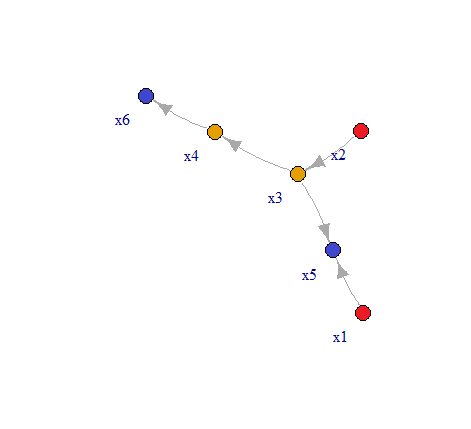
\includegraphics[scale=0.6]{bilder/Sufficient1_Graph.png}
	
%	\caption{Example network. Measured knots $x_5$ and $x_6$, hidden input knots $x_1$ and 
%	$x_2$.}
%	\label{fig:Sufficient1_Graph}
%\end{figure}
\end{example}

\clearpage
\subsection{Necessary Condition}

\begin{definition}{}{}
	We define $\mathfrak{V}_0 := V_0\backslash \{0\}$ and
	\begin{equation}
	\mathfrak{V}_i := V_i \cap P^{-1}\mathfrak{V}_{i-1} \quad .
	\end{equation}
\end{definition}

\begin{lemma}{}{}
	If and only if $\mathfrak{V}_d \neq \emptyset $ for all integers $d$, then it is possible to 
	find a $\mathbb{R}^m$ valued sequence $(v_k)_{k\in\mathbb{N}_0}$ such that $v_0\neq 0$ and
	\begin{equation}
	\left[ v_k,v_{k-1},\ldots,v_0 \right] \in V_k 
	\quad \forall k\in\mathbb{N}_0 \quad .
	\end{equation}
\end{lemma}
\begin{proof}
%	Assume $\mathfrak{V}_k\neq \emptyset$ holds for all $k$. Then for any $k$ there exists a $\xi$ with the 
%	properties
%	\begin{enumerate}
%	\item $\xi \in V_k$
%	\item $P\xi \in \mathfrak{V}_{k-1}$ i.e. $P\xi in V_{k-1}$
%	\item $P^r \xi \in \mathfrak{V}_{k-r}$ i.e. $P^r \xi \in V_{k-r}$
%	\item $P^k \xi \in \mathfrak{V}_0$ i.e. $P^k \xi\in V_0$ and $P^{k}\xi \neq 0$
%	\end{enumerate}
%	thus we can define the sequence $v_k$ by the projections of $\xi$. \\		

	Assume for any integer $K$ we find a sequence with $[v_k,\ldots,v_0]^\text{T}\in V_k$ for all $k\leq K$ and 
	$v_0\neq 0$. Then 
	we see by definition $v_0\in \mathfrak{V}_0$. Now assume $[v_{k-1},\ldots,v_0]^\text{T}$ 
	in $\mathfrak{V}_{k-1}$ and $[v_k,\ldots,v_0]^\text{T}$ in $V_k$. Comparing with the definition shows 
	that also 
	$[v_k,\ldots,v_0]^\text{T}$ in $\mathfrak{V}_k$. Thus with $v_0\neq 0$
	\begin{equation}
	[v_k,\ldots,v_0]\in V_k \forall k \quad \Rightarrow \quad [v_k,\ldots,v_0]\in \mathfrak{V}_k
	\forall k \quad .
	\end{equation}
	
	Now assume we found a $\mathfrak{V}_K = \emptyset$ and $\mathfrak{V}_k \neq \emptyset$ for all $k<K$. 
	If there was a sequence of $v_k$ such that $[v_k,\ldots,v_0]^\text{T}\in V_k$ and $v_0\neq 0$ for all $k<K$,
	then \\$[v_{K-1},\ldots,v_0]^\text{T}\in\mathfrak{V}_{d-1}$. By assumption there is no $\xi\in V_d$ 
	with the property $P\xi \in\mathfrak{V}_{d-1}$. Thus there cannot be such a sequence. 
\end{proof}

\begin{proposition}{Necessary Condition}{}
	If $\mathfrak{V}_d\neq \emptyset $ for all $d\in\mathbb{N}_0$, then we can find a nonzero function 
	$w:I\to\mathbb{R}^m$ on an nonvanishing interval $I$ such that $y\equiv 0$ on $I$.
\end{proposition}
\begin{proof}
	By lemma 4 we know there is a sequence $v_k$ such that $v_0 \neq 0$ and
	\begin{equation}
	\left[ v_k , v_{k-1},\ldots , v_0\right]^\text{T} \in V_k \quad .
	\end{equation}
	Thus if we define
	\begin{equation}
	w(t):= \sum\limits_{l=0}^\infty \frac{t^l}{l!} v_l
	\end{equation}
	we get $w^{(k)}(0)=v_k$ and $W^{(k)}(0)=[v_k,v_{k-1},\ldots,v_0]\in V_k$. If we expand $y(t)$ around 
	$t=0$ we get 
	\begin{equation}
	y(\tau) = y(0) + \sum\limits_{r=0}^\infty \frac{\tau^{r+1}}{(r+1)!} y^{(r+1)}(0)  
	= y(0) + \sum\limits_{r=0}^\infty \frac{\tau^{r+1}}{(r+1)!} \underbrace{M_r W^{(r)}(0)}_{=0} \equiv 0
	\end{equation}
	as long as $y$ can be expressed by its Taylor-expansion. \\
	
	Note that since $v_0\neq 0$, we know that $||[v_k,\ldots,v_0]^\text{T}||^2$ cannot converge to zero as 
	$k$ increases.  
\end{proof}	

\clearpage

\subsection{HIO Theorem}
\begin{proposition}{}{}
	To combine the necessary and sufficient condition, the implications
	\begin{equation}
	\mathfrak{V}_d \neq \emptyset \forall d\in\mathbb{N}_0 \quad \Longrightarrow \quad \mathfrak{O}_d 
	\neq \{0\}\forall d\in\mathbb{N}_0
	\end{equation}
	equivalently
	\begin{equation}
	\exists K \in\mathbb{N}_0 \big| \mathfrak{O}_K = \{0\} \quad \Longrightarrow \quad 
	\exists N \in\mathbb{N}_0 \big| \mathfrak{V}_N = \emptyset
	\end{equation}
	hold.
\end{proposition}
\begin{proof}
	First assume all $\mathfrak{V}_d$ are nonempty and we found a $\mathfrak{O}_N=\{0\}$. Then by the sufficient 
	condition we know that there cannot be a function $w$ such that $W^{(q)}(0)\in V_q$ for all $q$, but by the 
	necessary condition we know that we can construct such a function.\\
	
	The second implication is the complementary version of the first one.
\end{proof}

\begin{theorem}{}{}
	If and only if we can find a $\mathfrak{V}_d = \emptyset$, then
	\begin{equation}
	y\equiv 0 \quad \Rightarrow \quad w^{(q)}(0)=0\quad \forall q\in\mathbb{N}_0 \quad .
	\end{equation}
	If there are intervals $I_i$ such that $\overline{\bigcup I_i}=[0^-,T^+]$ and such that 
	$w$ can be represented by its Taylor-Expansion on each interval then
	\begin{equation}
	\exists d\in\mathbb{N}_0 \mathfrak{V}_d = \emptyset \quad \Longleftrightarrow \quad \text{HIO} \quad .
\end{equation}		
\end{theorem}
\begin{proof}
	Proposition 2 already shows, that if we cannot find an empty $\mathfrak{V}_d$, then we can construct a 
	function $w$ such that $y\equiv 0$ on an interval, where its Taylor series converges. Thus the existence of 
	such an empty $\mathfrak{V}_d$ is necessary for the implication.\\
	 
	Assume we found an empty $\mathfrak{V}_K$. By proposition 3 we know there is an $\mathfrak{O}_N=\{0\}$ 
	which is sufficient to show that $w$ must be a function such that $W^{(q)}(0)=0$ for all $q$. Thus the 
	existence of such a $\mathfrak{V}_K$ is also sufficient. \\
	
	Now assume there are intervals as in the theorem. 
	We write $t_i$ for the supremum of 
	$I_i$ and without loss of generality we can assume that the infimum of $I_{i+1}$ 
	coincides with $t_i$. 
	Then 
	\begin{equation}
	w^{(q)}(0) = 0 \forall q\in\mathbb{N}_0  \quad \Leftrightarrow \quad w\equiv 0 
	\text{ on }I_1 \quad .
	\end{equation}
	We now simply shrink the time domain to $[t_i^-,T^+]$ and straight forwardly get 
	\begin{equation}
	w^{(q)}(t_i) = 0 \forall q\in\mathbb{N}_0  \quad \Leftrightarrow \quad w\equiv 0
	\text{ on } I_{i+1}
	\end{equation}
	which means $w$ is the zero function on each interval. 
	Therefore $w\equiv 0$ on $[0,T]$.
\end{proof}
%
%
%\clearpage
%\subsubsection{Sufficient Condition 2}
%\begin{lemma}{}{}
%	Initialization:
%	\begin{equation}
%		y\equiv 0 \text{ in a vicinity of $t=0$} \quad \Rightarrow \quad 
%		w^{(0)} \in \mathfrak{D}_0 \quad .
%	\end{equation}
%	Induction step:
%	\begin{equation}
%	y\equiv 0 \text{ in a vicinity of $t=0$ and} W^{(q)}\in\mathfrak{D}_q \quad \Rightarrow 
%	\quad W^{(q+1)} \in \mathfrak{D}_{q+1} \quad .
%	\end{equation}
%\end{lemma}
%\begin{proof}
%	As already shown, $W^{(q)}(0)\in V_q$. Since $W^{(0)}=w^{(0)}$ and $V_0 = 
%	\mathfrak{D}_0$ the initialization is proved.\\
%	Now assum $W^{(q)}(0)\in\mathfrak{D}_q$. We know that $W^{(q+1)}\in V_{q+1}$ and 
%	therefore 
%	\begin{equation}
%	W^{(q+1)}(0) = [w^{(q+1)}(0),W^{(q)}(0)]^\text{T} \in 
%	V_{q+1} \cap P^{-1}\mathfrak{D}_q \quad .
%	\end{equation}
%	Note that $ P^{-1}\mathfrak{D}_q =\mathbb{R}^{m}\times \mathfrak{D}_q $ is just the 
%	assumption $W^{(q)}\in\mathfrak{D}_q$. The intersection $V_{q+1}\cap 
%	P^{-1}\mathfrak{D}_q = \mathfrak{D}_{q+1}$ was already shown in the remark hence
%	\begin{equation}
%	W^{(q+1)}(0) \in \mathfrak{D}_{q+1} \quad .
%	\end{equation}
%\end{proof}
%
%\begin{corollary}{}{}
%	As a direct consequence of the previous lemma
%	\begin{equation}
%	W^{(q)}(0) \in \mathfrak{D}_q \quad \forall q\in \mathbb{N}_0 \quad .
%	\end{equation}
%\end{corollary}
%\begin{proof}
%	It is a inductive proof with initialization and induction step as in the lemma.
%\end{proof}
%
%
%\begin{proposition}{Sufficient Condition 2}{}
%	If there is an integer $K$ such that $\mathfrak{D}_K = \{0\}$, then
%	\begin{equation}
%	y\equiv 0 \quad \text{in a vicinity of $t=0$} \quad 
%	\Rightarrow w^{(q)}(0) = 0 \quad \forall \quad q\in\mathbb{N}_0 \quad .
%	\end{equation}
%\end{proposition}
%\begin{proof}
%	Let $y\equiv 0$ and assume we have found an integer $K$ and 
%	$\mathfrak{D}_K=\{0\}$.
%	Then as already shown $W^{{K}}\in \mathfrak{D}_K$ implies 
%	\begin{equation}
%	W^{{K}}(0) = 0 \quad .
%	\end{equation}
%	If we now introduce a new integer $q\in\mathbb{N}_0$ we again get
%	\begin{equation}
%	M_{q+1+K} W^{(q+1+K)}(0) = 0 \quad \forall q\in\mathbb{N}_0
%	\end{equation}
%	which simplifies to
%	\begin{equation}
%	M_q \begin{bmatrix} w^{(K+1+q)}(0) \\ \vdots\\w^{(K+1)}(0) \end{bmatrix} = 0 \quad .
%	\end{equation}
%	As in the sufficient condition 1 this is equivalent to the equations before, but 
%	starting with $w^{K+1}$ as the lowest derivative. We straight forwardly deduce\\
%	$[w^{(K+1+q)}(0),\ldots,w^{(K+1)}(0)]^\text{T}\in \mathfrak{D}_q$ which implies that 
%	\begin{equation}
%	W^{(2K)}(0) \in \mathfrak{D}_K \times \mathfrak{D}_K = \{0\} \quad .
%	\end{equation}
%	This shows that we can do an inductive proof to show
%	\begin{equation}
%	W^{(rK)}(0) \in (\mathfrak{D}_K)^{\times r} \quad \Rightarrow \quad  
%	W^{((r+1)K)}(0) \in (\mathfrak{D}_K)^{\times (r+1)}
%	\end{equation}
%	to get 
%	\begin{equation}
%	W^{(rK)}(0) = 0 \quad \forall r\in\mathbb{N}_0
%	\end{equation}
%	which means $W^{(q)}(0)=0$ for any integer $q$ and thus $w^{(q)}(0)=0$. 
%\end{proof}
%
%\begin{remark}{}{}
%	Note, that there are some important differences between condition 1 and condition 2.
%	\begin{enumerate}
%	\item The sequence $\mathfrak{O}_q$ converges in finite dimensions whereas 
%	$\mathfrak{D}_q$ approaches a subspace of the infinite dimensional space of sequences.
%	\item The equation $P^q \mathfrak{D}_q = \mathfrak{O}_q$ holds for all 
%	$q\in\mathbb{N}_0$. Therefore $\mathfrak{D}_K=\{0\}$ implies $\mathfrak{O}_q=\{0\}$ and 
%	hence condition 1 covers more cases than condition 2. E.g. the latter example 
%	fulfils condition 1 but not condition 2. 
%	\end{enumerate}
%\end{remark}
%
